\documentclass[preprint]{iucr}
 \journalcode{J}
 \papertype{CP}

\usepackage{graphicx}
\usepackage{minted}

\usepackage[T1]{fontenc}
\usepackage[utf8]{inputenc}

\begin{document}

\title{The Fast Azimuthal Integration Python library}
\shorttitle{PyFAI}

    \author[a]{Aurore}{Deschildre}
    \author[a]{Giannis}{Ashiotis}
    \author[b]{Zubair}{Nawaz}
    \author[a]{Jonathan P.}{Wright}
    \author[a]{Dimitrios}{Karkoulis}
    \author[c]{Fr\'ed\'eric-Emmanuel}{Picca}
    \cauthor[a]{J\'er\^ome}{Kieffer}{jerome.kieffer@esrf,fr}{}
    \aff[a]{European Synchrotron Radiation Facility, 71 Avenue
    des Martyrs, \city{Grenoble},
    \country{France}}
    \shortauthor{Kieffer et al.}

\maketitle

\begin{synopsis}
Details about the geometry, peak-picking, calibration and integration procedures
on multi- and many-core devices implemented in the Python library for high
performance azimuthal integration.
\end{synopsis}

\begin{abstract}
PyFAI is an open source software package designed to perform azimuthal and
radial integration and, correspondingly, 2D regrouping on area detector frames for small and wide
angle X-ray scattering experiments.
It is written in Python, a language widely accepted and used by the scientific
community today, which enables the users to easily incorporate the PyFAI
library into their processing pipeline.
This contribution focuses on recent work, especially the ease of
calibration, its accuracy and the execution speed for integration.
\end{abstract}

\section{Introduction}
Azimuthal integration allows the usage of area detectors for recording powder
diffraction patterns, which  ensure larger solid angle coverage and hence a
better harvest of X­-ray photons.
This data reduction step is often one of the most time ­consuming tasks in the
processing pipeline and sometimes limits the productivity of modern synchrotron
beamlines, where diffraction is used to probe samples with a point focussed
beam in 2D raster scans or diffraction tomography experiments and
very fast detectors.

This contribution describes the Python library pyFAI in its version 0.10
(released in october 2014) which can be used to calibrate the experimental
setup of a powder diffraction experiment or a SAXS experiment using area
detector using Debye-Scherrer rings collected from a reference compound.
After describing how the geometry is internally represented in pyFAI, the
various image analysis algorithm used to extract Debye-Scherrer rings are presented.
Those peaks positions are combined with the knowledge of a calibrant and the
wavelength of the radiation to perform the refinement of the detector position
in space.

Once this geometry is known, azimuthal regrouping can be performed.
As pyFAI implements various algorithm for integration, including
multiple pixel splitting schemes, they will be exposed and compared
for speed, precision and memory consumption.
A scientific example is given on how pyFAI can be used to decompose
diffraction images into amorphous and Bragg components and its application
to serial crystallography.

As pyFAI is a library, and many users prefer an integrated graphical user
interfaces (GUI), some other project related to pyFAI are described before
concluding.

Appendices contains information about the project structure, precision
on how to calibrate an experimental setup and precisions on the many-core
implementation of azimuthal integration using OpenCL \cite{opencl}.

\section{Experiment description}
In pyFAI, a basic experiment is defined by an area-detector whose position
in space is defined from the sample position and the incident radiation.

\subsection{Detector}
Like most other diffraction processing packages, pyFAI allows the definition of
2D detectors by a constant pixel size (in meter) but this approach shows its limits
with different types of detectors, especially multi-module detectors and fiber
optic taper coupled detectors. Large area pixel detector are often composed from
the assembly of smaller modules (i.e. Pilatus from Dectris, Maxipix from ESRF,
\ldots).
By construction, such detector exhibit gaps between modules and pixels of
various sizes within a single module, hence they require a specific mask.
Optically coupled detectors need also to be corrected
for small spatial displacement, often called geometric distortion.

\subsubsection{Detectors classes} are used to define a family of detectors.
To take the specificities of each detector into account, pyFAI contains about
40 detectors class definitions which contain the mask (invalid pixels,
gaps, \ldots) and a method to calculate the pixel position in cartesian coordinates.
For optically coupled CCD detectors, the geometrical distortion is often
described by a bi-dimensional cubic spline which can be imported into
the detector instance and used to calculate the actual pixel position in space.

\subsubsection{Nexus Detectors:}
Any detector object in pyFAI, can be saved to a HDF5 file following the NeXus
\cite{nexus} convention.
Detector objects can subsequently be restored from the disk, making
complex detector definition less error-prone.
Pixels of an area detector are saved as a 4-dimensional dataset: 2D
array of vertices pointing to every corner of each pixel, which makes an array
of shape: ($Ny$, $Nx$, $Nc$, 3) where $Nx$ and $Ny$ are the dimension of the
detector, $Nc$ the number of corners of each pixel, usually 4, and the last
dimension contains the vertex itself.
This definition, while relying on large description file,
can address some of the most complex detectors layout:
\begin{itemize}
  \item hexagonal pixels (i.e. Pixirad detectors)
  \item curved /bent imaging plates (i.e. Rigaku)
  \item tiled modules pixel detectors (i.e. Xpad detectors from ImXpad)
  \item semi-cylindrical pixel detectors (i.e. Pilatus12M from Dectris).
\end{itemize}

\subsection{Geometry}
The experiment geometry is defined in pyFAI by the position of the detector in
space, the origin being located at the sample position, more precisely where the
X-ray beam crosses the diffractometer's main axis (figure \ref{PONI}.
The detector being a rigid body, its position in space is described by
six parameters: 3 coordinates and 3 rotations.
In pyFAI, we use the point, orthogonal projection
of origin on the detector surface (Z=0 in detector's coordinate system, for
non planar detecors), called PONI (for Point Of Normal Incidence, \cite{spd}).
The detector distance is the sample-PONI distance
and the PONI coordinates are measured in the detector's referential (origin at the lower
left of the image). As pixel size could be non constant, all 3 distances are
given in meter.
The 3 rotations, stored in radians, correspond to the rotation along the 3
axes.

\begin{figure}
\label{PONI}
\begin{center}
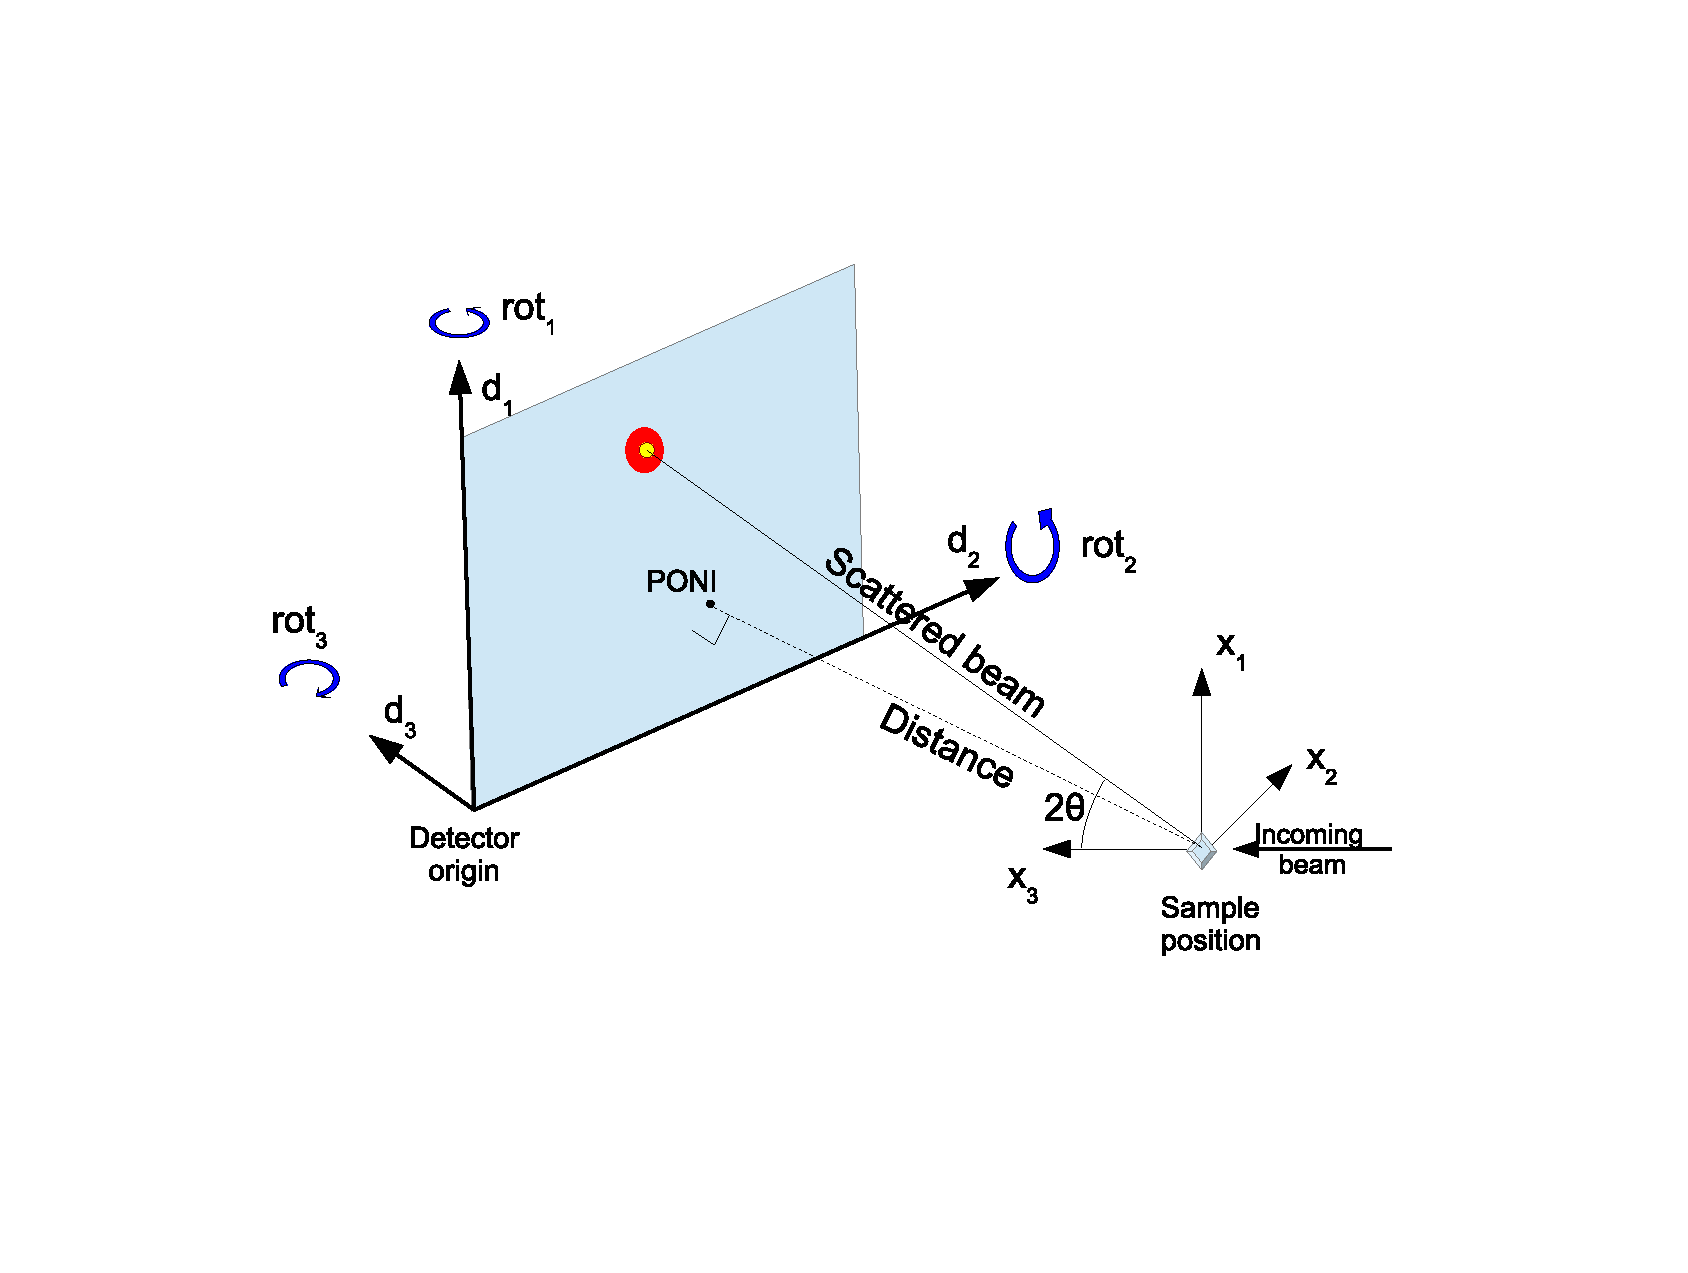
\includegraphics[width=15cm]{PONI.eps}
\caption{Geometry used by pyFAI}
\end{center}
\end{figure}

When all rotations are zero, the detector is in transmission mode with the
incident beam orthogonal to the detector's surface.
The choice of S.I. units may look unadapted or odd to users familiar to
other code like FIT2D \cite{fit2d}, therefore the geometry used in pyFAI can be
exported to and imported from the parameter sets from other software.
We are happy to integrate geometries used in other software to ease the
comparison of results and cross-validate approaches.

\subsubsection{Binning}
One of the strength of this geometry is capability to perform binning of the
detector without having to re-calibrate or re-calculate the position in space.
All pyFAI detector classes have a binning option which will increase the pixel
size accordingly and divide detector shape accordingly.
This even works for detectors with distortions (as the spline can be
evaluated on various grid size).

\section{Calibration}
Calibration of the position of the detector is performed using Debye-Scherrer
rings collected from a reference powder called ``calibrant''.
Rings are extracted (see \ref{massif}) and control points are located as maxima
of those rings.
The geometry of the experiment is obtained from a least-squares refinement of
the $2\theta$ angles.
In this contribution we will call them ``ring'' even if, for planar detector,
they are actually conics formed by the intersection of the Debye-Scherrer cones
with the detector plan.
PyFAI does not assume rings are circles, ellipses or parabolas and is able to
fit the geometry of a wide range of experiments.
The support for the geometry refinement of non planar detectors is still under
development.

\subsection{Calibrant}
PyFAI provides ten calibrant descriptions among the most used ones: ceria,
corundum, gold, lanthanum hexaboride and silicon for powder diffraction;
silver behenate, tetradecanol and para-bromobenzoic acid for small angle scattering.
Any file containing d-spacing in angstrom can be used as calibrant for a
geometry calibration and can be loaded by the \textit{Calibrant} class instance.
This \textit{calibrant} object is in charge of
calculating the reference $2\theta$ cone aperture
against which the geometry will be refined (provided the wavelength/energy is
known).

\subsection{Peak-picking}
With micro and nano-focused beams available on modern synchrotron facilities
\cite{id13}, fewer crystals get hit by the beam going through the
sample making Debye-Scherrer ring obtained from the diffraction of reference
powders spotty.
As grinding reference powder is not advised (it would at least broaden peaks
and may introduce strain), we decided to
address this issue by image analysis and reconstruction of Debye-Scherrer rings.
An alternative approach is to use single crystal indexation techniques for
example using the Fable software \cite{fable} as demonstrated for diffraction
tomography experiment \cite{bonnin}.

\subsubsection{``Massif'' extraction}
\label{massif}
allows a clear separation between regions containing large
photon counts (rings) and the background.
It uses a difference of the image with itself, Gaussian blurred with a given
width, $\sigma$.
Border of the regions with high intensity (\textit{massif}) are negative in this
difference image, so positive regions are labeled and represent
(a fraction of) a ring. Peaks, which are local maxima,
are sampled within the same region and belong to the same ring.
The width of the Gaussian, in pixel units, has to be larger than the typical
distance between two peaks within a ring and smaller than the distance between two
rings.
PyFAI includes some heuristics to guess an acceptable parameter in most cases
but they can be overridden by the command line argument \textit{--gaussian=XX},
where XX is the size of the gaussian in per-mille of the image size.

\subsubsection{Sub-pixel precision}
\label{subpixel}
on the peak position is obtained using a second order development of the
intensity on the neighborhood of the peak position $\overrightarrow{x_0}$:
$$ I(\overrightarrow{x}) = I(\overrightarrow{x_0}) + \nabla
I(\overrightarrow{x_0})\cdot (\overrightarrow{x}-\overrightarrow{x_0}) +
\frac{1}{2} (\overrightarrow{x}-\overrightarrow{x_0})^T\cdot\mathcal{H}
I(\overrightarrow{x_0})\cdot(\overrightarrow{x}-\overrightarrow{x_0})$$ which
can be derived into:
$$\nabla I(\overrightarrow{x}) =\nabla I(\overrightarrow{x_0}) +
\mathcal{H}I(\overrightarrow{x_0})\cdot(\overrightarrow{x}-\overrightarrow{x_0})$$
The position of the actual maximum $\overrightarrow{x}$ is define by
$\nabla I(\overrightarrow{x})=0$, hence:
$$\overrightarrow{x} = \overrightarrow{x_0} - (\mathcal{H}
I(\overrightarrow{x_0}))^{-1}\cdot\nabla I(\overrightarrow{x_0})$$ where $I$,
$\nabla I$ and $\mathcal{H} I$ are the scalar field of intensity, its gradient
(vector) and Hessian (matrix), respectively, measured at the maximum pixel position.
Those derivatives are numerically assessed on a 3x3 neighborhood, so with noisy
data, it happens that $\overrightarrow{x}$ is far away from
$\overrightarrow{x_0}$ (more than a pixel). In such cases, $\overrightarrow{x}$
is taken as the center of mass of the 3x3 neighborhood around
$\overrightarrow{x_0}$ (less precise, but more robust).

\subsubsection{Blob detection}
\label{blob}
is a computer vision method which allows to perform peak-picking without
\textit{a priori} knowledge on the level of the image.
This feature is essential to us as diffraction images exhibit a very large
dynamic range.

The diffraction image is sequentially blurred with Gaussian filters which
width $\sigma$ follows the geometric series: $\frac{1}{2}$,
$\frac{\sqrt{2}}{2}$, 1, $\sqrt{2}$, 2, $2\sqrt{2}$, \ldots
For each blurred image at scale $\sigma$, the subsequent blurred (at
$\sigma'=\sigma\cdot\sqrt(2)$
is subtracted to create a difference of Gaussian
image (called $DoG$) which highlights the features of the image which typical
size is $\sigma$.
A 3D scale-space ($x,y,\sigma$) representation is created from those DoG images.

This method provides us not only the peaks location, as local maxima in
scale-space, but also the typical size of the peak.
Peak position, scales and intensity are refined as described in
\ref{subpixel}, extended to the 3D scale space.

To keep the computation time reasonable, the implementation of the blob
detection relies on Gaussian convolution in real space (i.e. without Fourier
transform), separated in horizontal and vertical direction, with small
convolution kernels of width $8 \sigma +1$.
To prevent the growth of the window with larger $\sigma$, a pyramid of Gaussians
is built by binning the blurred image by a factor 2 when it reaches a
$\sigma=2$.

The drawback of this algorithm, beside the calculation time, is its very high
sensitivity to noise in flat regions.
This is why blob detection is only used in the re-calibration procedure to
extract all peaks in a region of interest, determined form an
approximative geometry.
Moreover blob detection cannot find peaks wich width is smaller than
$\sigma=0.7$ which correspond to 3 pixels.


\subsection{Graphical user interface for calibration}
Only a minimalistic graphical user interface (called
\textit{pyFAI-calib}, figure \ref{calib}) is provided
for peak-picking, with visual assignment of the ring number.
An rough estimate of the geometry is usually obtained from a mouse click on
two of the inner-most rings.
The pink and yellow dots correspond to the control points (peaks) extracted
using the algorithm described in \ref{massif} (with only two mouse clicks).
The refinement is performed on the error in $2\theta$ (squared) using the
Sequential Least SQuares Programming  from
SciPy (function \textit{scipy.optimize.min\_slsqp}).
After refinement of the geometry, the iso-contour for refined $2\theta$ array is
overlaid to the diffraction image. Those are the four thin plain lines drawn on
the image to mark where Debye-Scherrer rings are expected, allowing a visual
validation of the calibration.

\begin{figure}
\label{calib}
\begin{center}
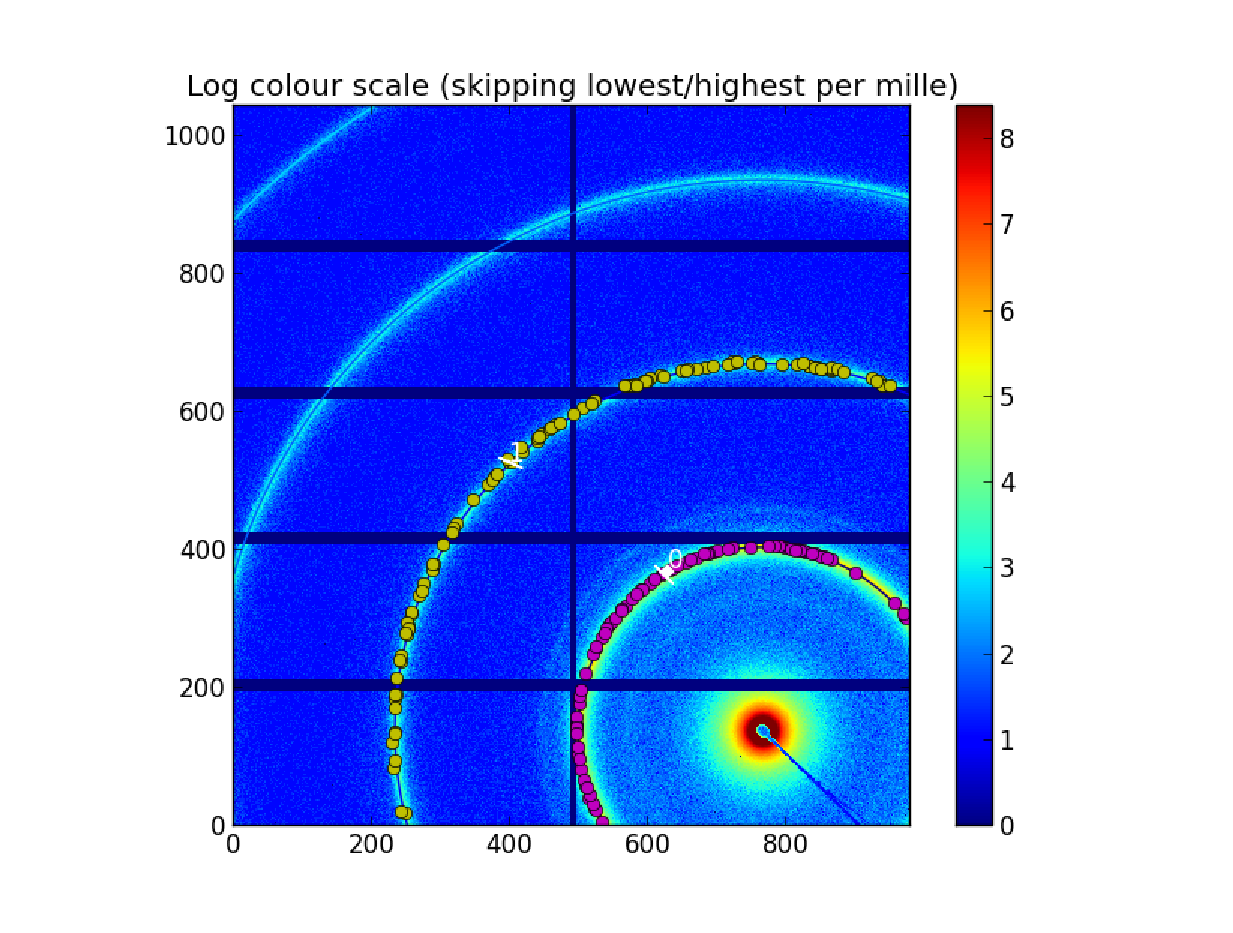
\includegraphics[width=15cm]{calib.eps}
\caption{The calibration window allows manual peak-picking and
ring assignment. The data correspond to a silver behenate sample, used as a
calibrant on the BioSAXS beamline BM29 at the synchrotron ESRF
(detector: Pilatus 1M, $\lambda=1.0${\AA})}
\end{center}
\end{figure}

From this initial rough calibration, pyFAI allows to perform many operations in
Command Line Interface (CLI) mode, like setting, constaining, fixing and
refining parameters, extracting a new set of keypoints or performing the
integration. The complete description of options is described in annex
\ref{annex_calib}.

\section{Azimuthal Integration}

The core of pyFAI is to be able to perform azimuthal integration in 1D or 2D as
fast as possible, using Python binary extensions, often multi-threaded or even
mani-core accelerated (i.e. Graphics Processors Units, GPU and Intel Xeon
Phi accelerators), while offering a common interface at the Python level.
Many details on the techniques used to speed up the code, especially porting
it to GPU have been described in \cite{kieffer_ashiotis-proc-euroscipy-2014}.

\subsection{Programming interface for azimuthal integration}

The initial idea behind pyFAI is to provide a easy way to perform azimuthal
integration, ideally in a single command. In the snippet of code we present how
this is done:

%\begin{verbatim}
\begin{minted}{python}
import pyFAI, fabio, pylab
img = fabio.open("imagefile.tif").data
ai = pyFAI.load("geometry.poni")
tth, I = ai.integrate1d(img, 1000, unit="2th_deg", method="splitpixel")
pylab.plot(tth, I)
pylab.show()
\end{minted}
%\end{verbatim}

The fist line load three important libraries: fabio \cite{fabio} to read
images, pylab \cite{matplotlib} to display the result and pyFAI.
The second and third line load the image and the geometry.
the two last lines are about displaying the curve.

In this snippet, the image \textit{img} is azimuthaly integrated into 1000 bins with an
out, eventhly spaced in $2\theta$. Other units like the scattering vector length
$q$ or the radius $r$ are available.
The method keyword is a switch to select the algorithm used.

\subsection{Pixel splitting schemes and implementation}

PyFAI implementents a dozen of azimuthal integration procedures which can be
classified according to they way integration is performed and the pixel
splitting scheme used.

\subsubsection{Histogram vs Look-Up Table.}
The naive way to integrate data is to treat an image pixel after pixel,
implemented like an histogram. This is a scatter operation which is hard to
parallelize but cheap in memory.
Using a \textit{scatter to gather} transformation, the azimuthal integration for
a given geometry can be stored into a look-up table (LUT) and applied like a
sparse matrix, dense vector multiplication.
While much more expensive in memory, this
implementation is effective in parallelization and speed.
The Compressed Row Storage (CSR) matrix representation is now used in place of
the LUT and provides a lower memory footprint.

\subsubsection{Three pixel splitting} schemes are available in pyFAI and define
the way photons counted by a pixel are assigned to the various histogram bins,
especially when the pixels are large (Pilatus detectors):
\begin{itemize}
\item No splitting: the full intensity is assigned into a single bin (dirac
like shape)
\item Bounding box splitting: the pixel is abstracted by a simpler shape
oriented parallel to the radial and azimuthal directions.
\item
Tight/full pixel splitting: the only assumption made is that pixel
edges are lines.
\end{itemize}
The figure \ref{split} presents the way a single pixel is split on a
large number of bins using the three schemes exposed previously. The way Fit2D
splits pixels has been added for comparison: it looks pretty similar to bounding
box pixel splitting but the abstracted shape is likely to be smaller.

\begin{figure}
\label{split}
\begin{center}
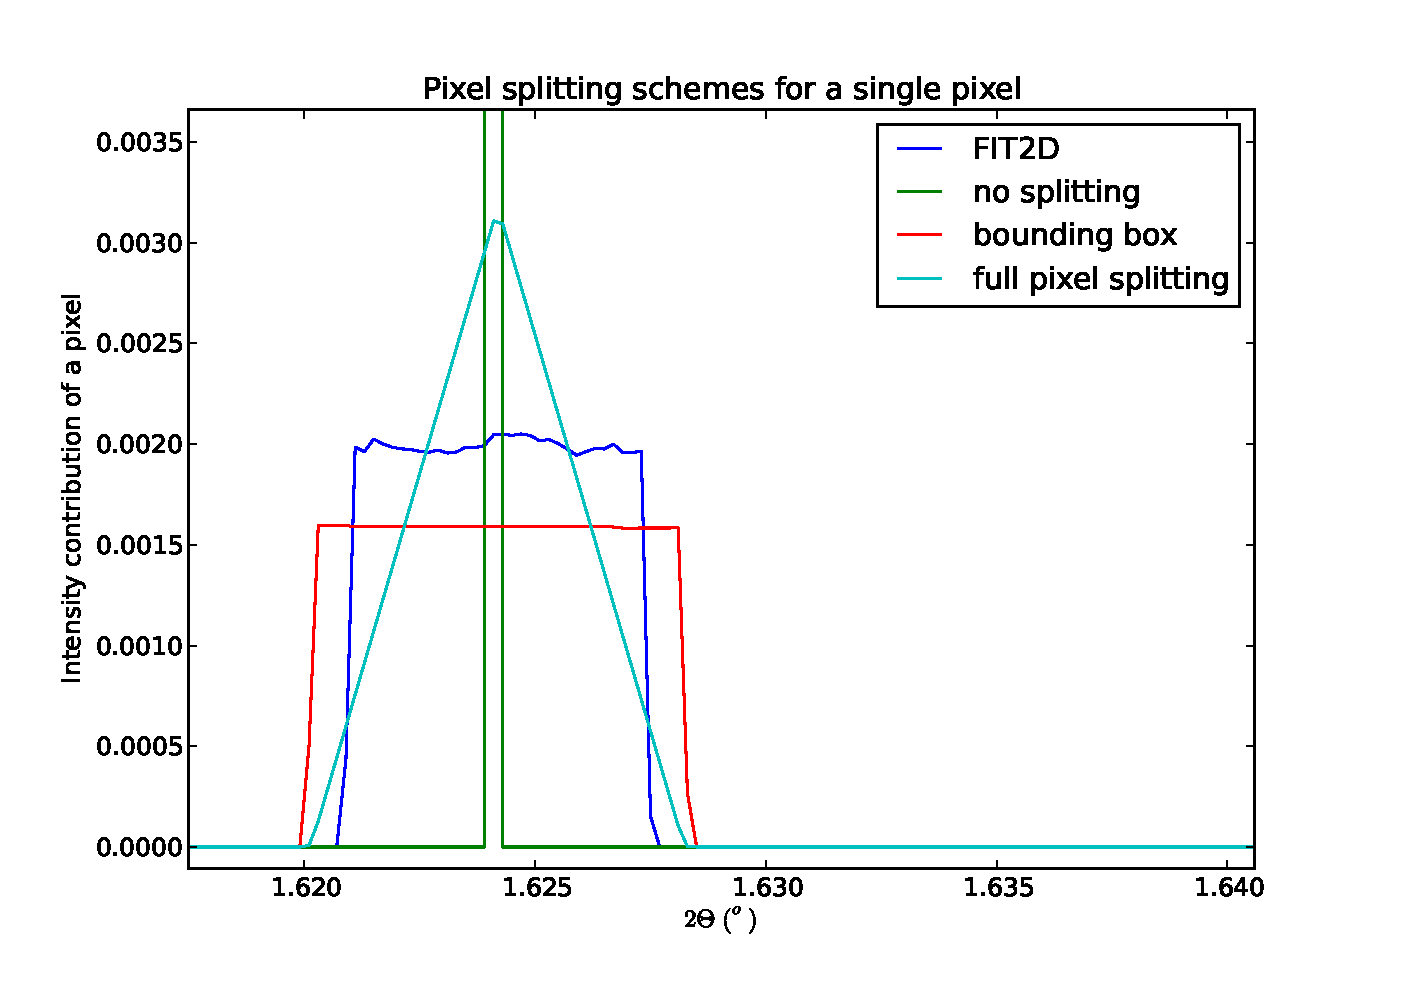
\includegraphics[width=15cm]{splitpixel.eps}
\caption{Contribution to a powder diffraction pattern of a single pixel to
highlight the pixel splitting algorithm underneath. PyFAI's implementations are
compared to FIT2D.}
\end{center}
\end{figure}

\subsubsection{Summary about speed and memory consumption.}

The table {table:methods}  summarizes the various implementation available
with their execution speed and the memory footprint for integrating a 2048x2048
pixels image into 1000 bins.

\begin{table}
\caption{Various ``methods`` available within pyFAI for azimuthal integration
featuring their speed and memory footprint. Measured on a 3 GHz quad-core
computer with a 2048x2048 pixels image.}
\begin{tabular}[pos]{|c|l|l|l|}
\hline
Pixel split& No splitting & Bounding box & Tight pixel \\
\hline
Direct    & numpy (889 ms, 336 MB) & splitbbox (129 ms, 343 MB) &
splitpixel(516 ms, 480 MB)\\
histogram & cython (361 ms, 323 MB) &                       &                \\
\hline
Look-up   &       & splitBBoxLUT (59 ms, 327 MB) &    \\
table     & CSR nosplit (48 ms, 330 MB)       & CSR bbox (52 ms, 330
MB) & CSR full (51 ms, 502 MB)\\
\hline
\end{tabular}
\label{table:methods}
\end{table}

It is worth mentioning that while pixel splitting provides smoother results, any
pixel splitting scheme introduces some serial-correlation between
neighboring bins, introducing an overestimation of errors, as described in \cite{billinge2014}.

\subsection{Graphical user interface for azimuthal integration}

A minimalistic user interface called \textit{pyFAI-integrate}, is
shown in figure \ref{pyFAI-integrate}.
It has most of the feature available in pyFAI:
the top frame contains the geometric description of the experiment.
The second frame is about correction to be applied: dark current subtraction,
flat-field correction, polarization and solid-angle effects, static and dynamic
masking. The checkboxes next to each field allows to activate (or not) the given
correction.
The third frame contains information about the output format, the number of bins
in radial and azimuthal dimensions togeather with the output space.
The last frame allows the use to run calculation on an OpenCL device and
chose it.

\begin{figure}
\label{pyFAI-integrate}
\begin{center}
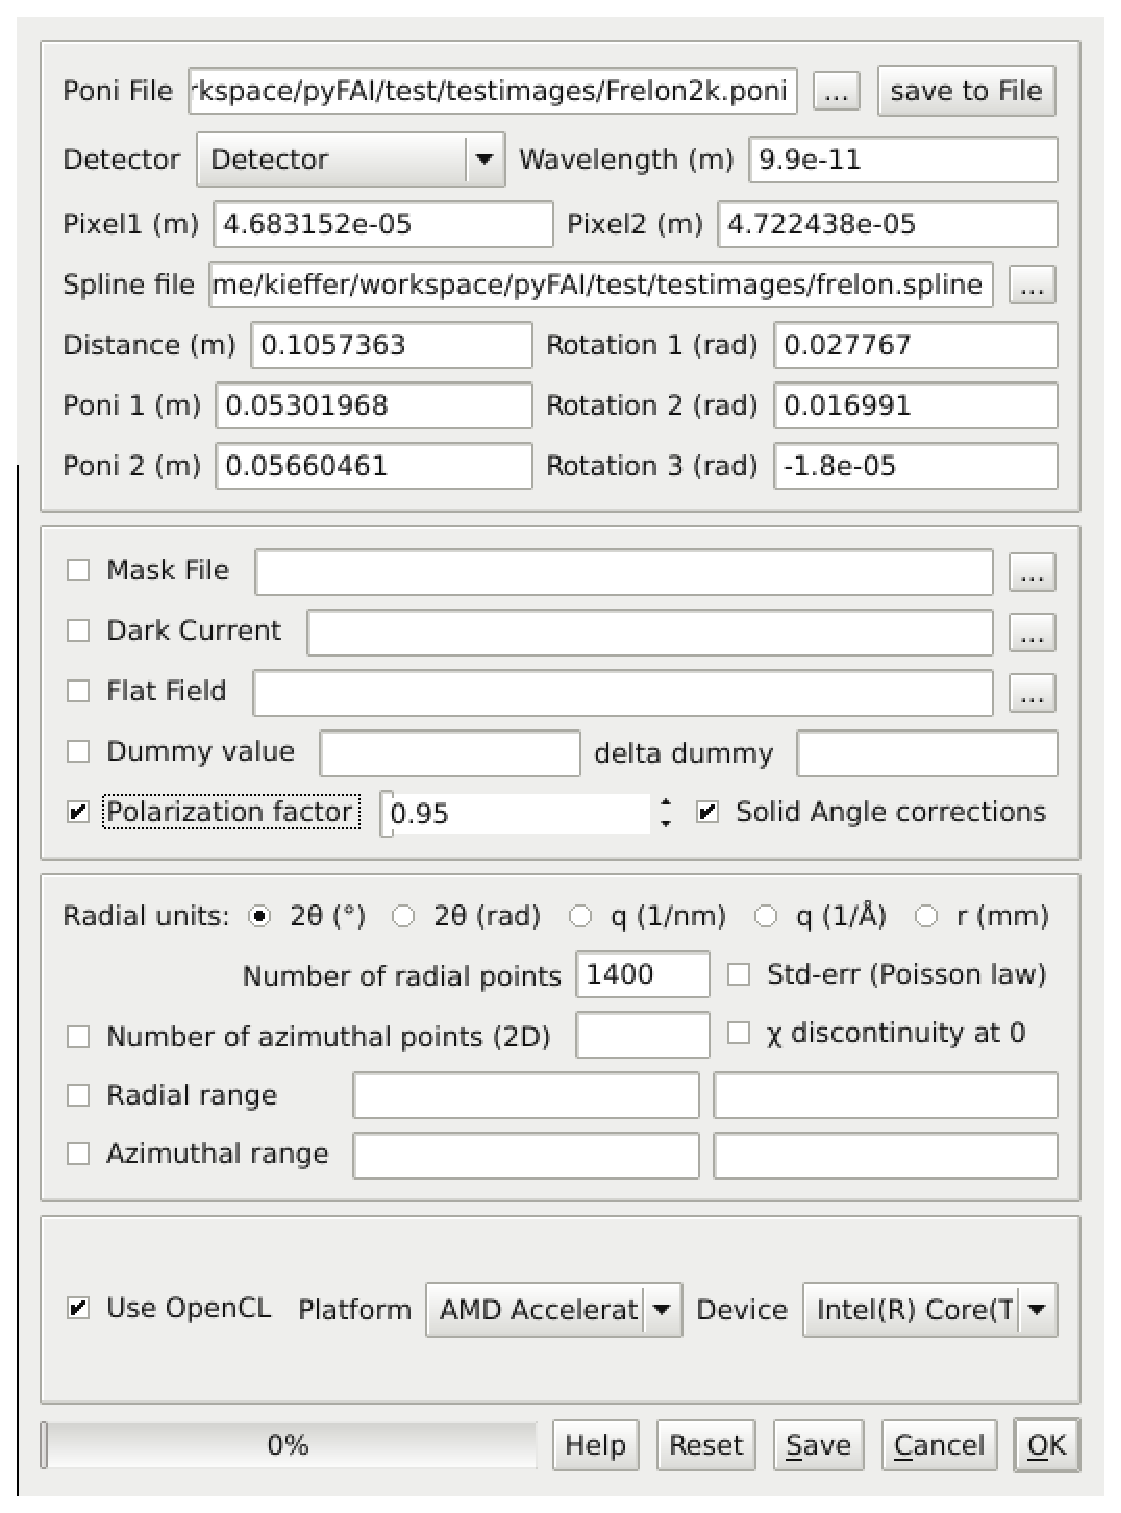
\includegraphics[width=15cm]{integrate.eps}
\caption{Graphical interface for performing azimuthal integration on a set of
images.}
\end{center}
\end{figure}

\section{Example of applications}

Azimuthal regrouping and its opposite transformation (assuming
uniform-distribution over the azimuthal angle) can be performed
using pyFAI which offers many opportunities for processing.

\subsection{Diffraction image generation}

Once the geometry defined (i.e. by loading a poni-file), the $2\theta$ and
$\chi$ position of every single pixel of the detector are known.
If one assumes the isotropy of signal (real powder without prefered
orientation), \textit{2D} diffraction patterns can be generated as exposed in this
example:

%\begin{verbatim}
\begin{minted}{python}
import numpy, scipy.signal, pyFAI
N = 1000 # generate the powder curve as a single gaussian
tth = numpy.linspace(0, 60, N)
I = scipy.signal.gaussian(N, 5)
det = pyFAI.detectors.detector_factory("Pilatus1M")
ai = pyFAI.AzimuthalIntegrator(dist=0.1, poni1=0.1, poni2=0.1, detector=det)
img = ai.calcfrom1d(tth, I)
\end{minted}
%\end{verbatim}


The method, \textit{calcfrom1d} is available from any
\textit{AzimuthalIntegrator} or \textit{Geometry} instance.
It is used together with a calibrant object to generate a fake diffraction image
suitable for testing pyFAI or other calibration codes (for example to validate
the geometry translation from one program to another).


%\begin{verbatim}
\begin{minted}{python}
import pyFAI.calibrant
lab6 = pyFAI.calibrant.ALL_CALIBRANTS["LaB6"]
lab6.set_wavelength(1e-10)
img_lab6 = lab6.fake_calibration_image(ai)
\end{minted}
%\end{verbatim}

In this snippet of code, a reference sample LaB$_6$ is defined on the second
line from the known calibrants before the the wavelength is set.
Combined with the geometry, this calibrant is able to
generate a 2D numpy array containing the simulated Debye-Scherrer diffraction
rings which can be saved or displayed on the screen.
The \textit{fake\_calibration\_image} contains further option to set U, V and W
parameters from Caglioti's formula \cite{caglioti} to include the
broadening of peaks according to this simple resolution function.
Calibrants in pyFAI contain only their \textit{d-spacing}, so the
reconstructed image will have all rings with the same
intensity (once integrated).

\subsection{Image offset and validation of the calibration}
By regenerating a 2D diffraction image from the integrated powder pattern one
can assess the quality of the calibration used for the integration.
The calibration tool, \textit{pyFAI-calib}, offers  a ``validate'' command which
measures the offset on the image (x, y) between the 2D diffraction image and the
one regenerated from the integrated patern, using a phase correlation
algorithm.
This allows a measurement of the precision of localization of the PONI, which
can be better than a tenth of a pixel, when calibrating images with continuous
rings (i.e. not spotty) with a mask large enough to remove the beam stop and
all parasitic scattering.

\subsection{Amorphous background removal}

PyFAI's azimuthal integrator features a \textit{separate} method able to separate
the background with an azimuthal symmetry (amorphous scattering or powder's
ring), from Bragg peaks automatically.

Based on what was described in \cite{PyFAI_PDJ}, a bidimensional azimuthal
integration is performed on the input image.
The output 2D image is filtered along the azimuthal $\chi$ axis using a
percentile (often median) filter to reconstruct the powder diffraction curve
without the sharp Bragg spots.
The number of points in azimuthal and radial direction as well as
the percentile value can be adjusted but the default values are reasonably
good.

The reconstructed 2D image corresponds to the amorphous/powder/isotropic
component of the input image and the subtraction of this generated image from
the raw data contains only the signal coming from large crystals.
Figure \ref{separate} (left)
presents a close-up of protein single crystal data recorded on a Pilatus3-2M
detectors (image taken at the ID23-2 beamline from ESRF). A
diffuse amorphous halo is clearly visible.
After using the automatic amorphous background removal, which takes into account
the mask needed for such pixel detectors, only Bragg peaks remain (right of
the image).

\begin{figure}
\label{separate}
\begin{center}
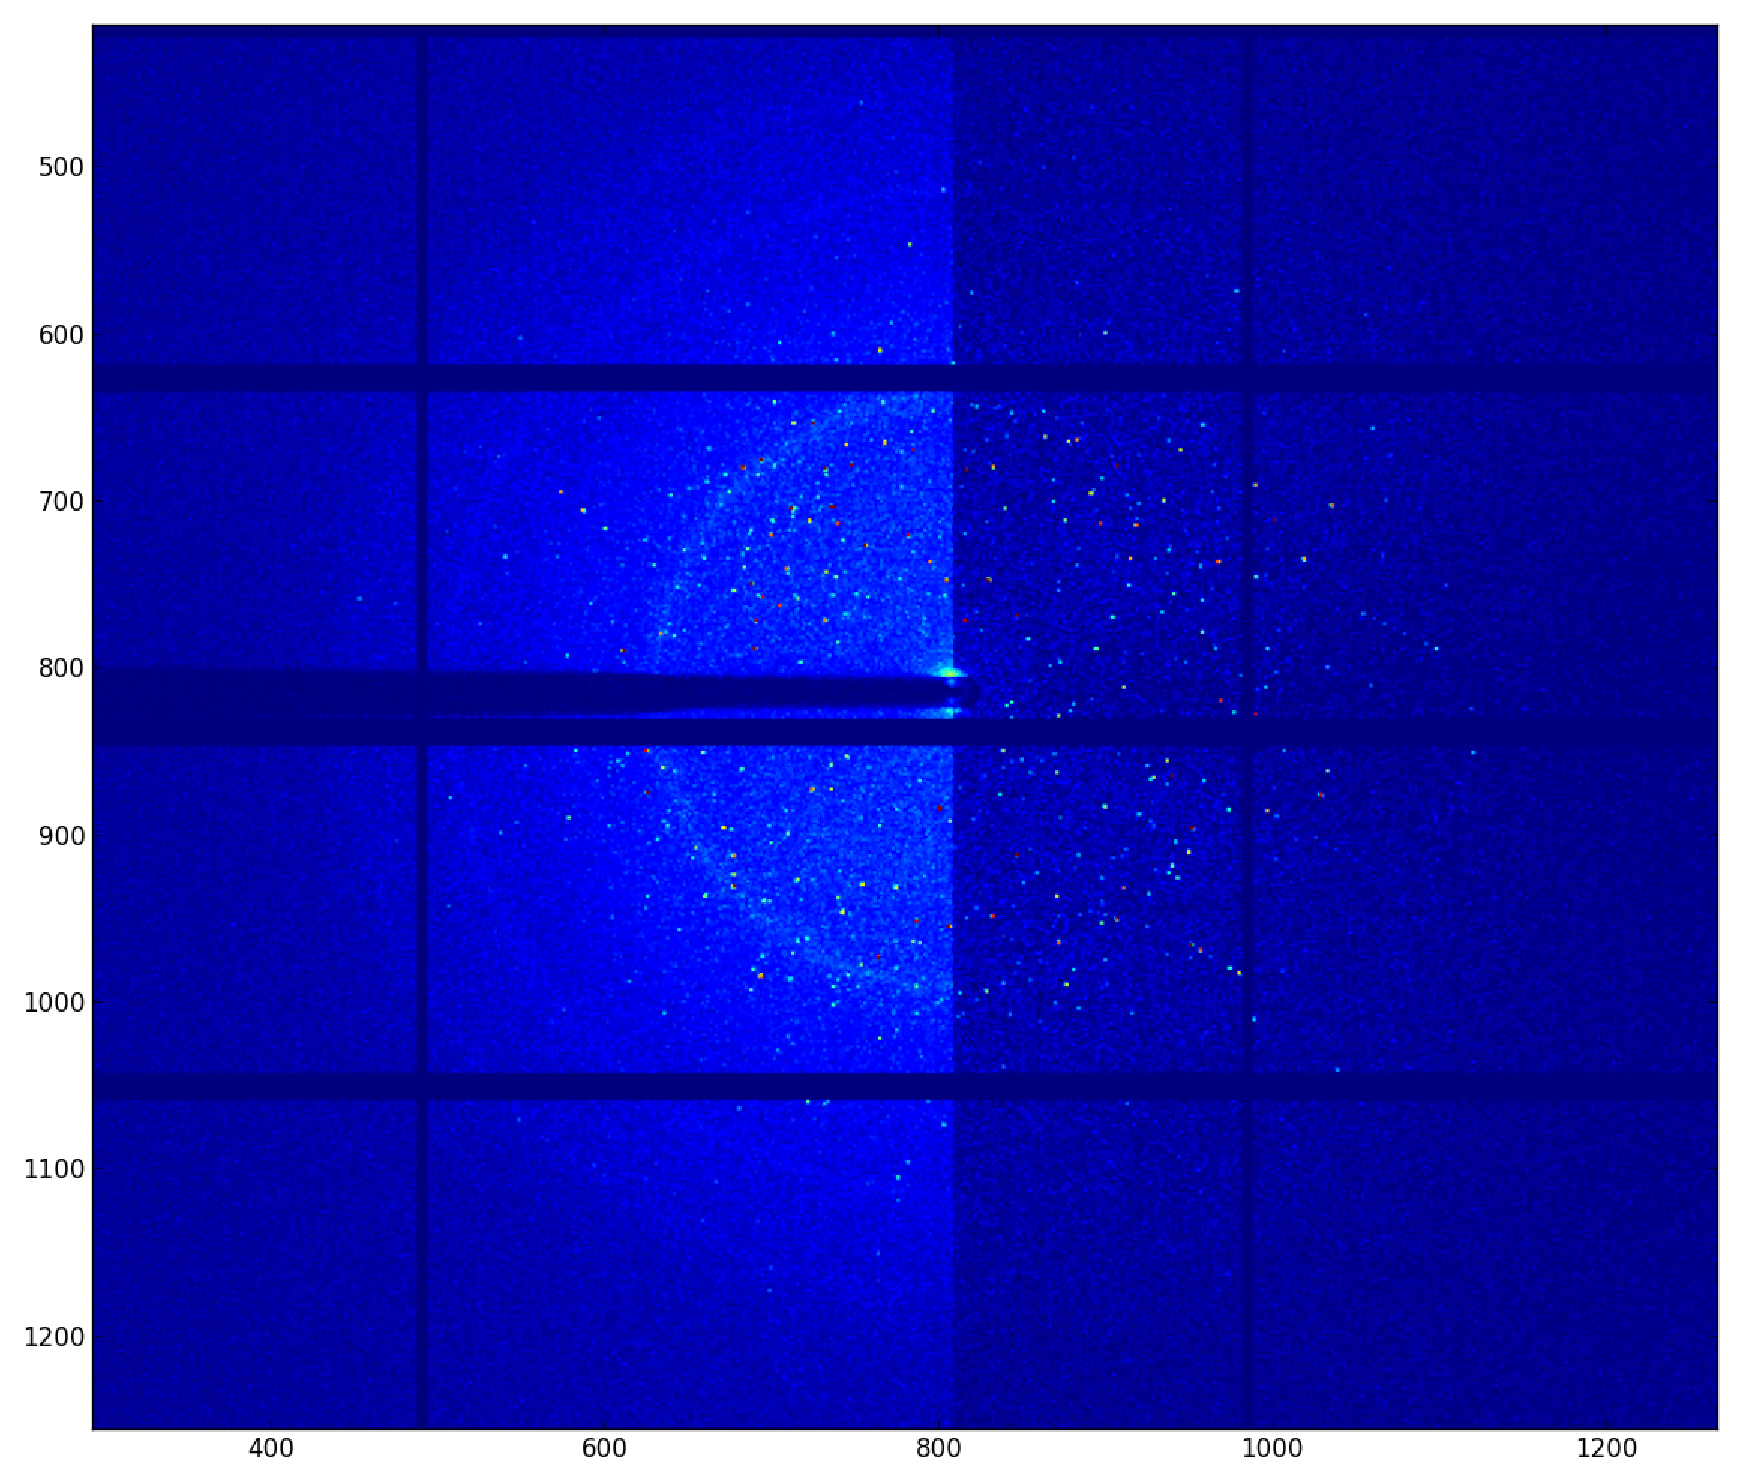
\includegraphics[width=15cm]{separate_id23.eps}
\caption{Automatic removal of amorphous signal (ice ring) from Bragg peaks in a
protein crystallography experiment (data from beamline ID23 at synchrotron
ESRF).}
\end{center}
\end{figure}

\subsubsection{Application to serial crystallography}
In these experiments, tiny crystals in their solvent are sent in
front of the X-ray beam (using a jet or moving a motor) and data are acquired
continuously, using a fast detector (from dozens of Hertz to kHz).
Those experiments produce a huge amount of data and only a small fraction of the
frames contain diffraction signal.
PyFAI has been integrated into the processing software \textit{NanoPeakCell}
which provides a graphical interface for frame selection in serial crystallography.
But pyFAI has also been integrated into the LImA data acquisition system
\cite{lima}, where it assesses the amount of single crystal
diffraction data within each frame and decides to save it or not.
In this way, a huge amount of disk space and network bandwidth
can be saved.

\section{Related Work}

As mentionned earlier, the pyFAI software library has been integrated
into other software, mainly integrated at the different beamlines from
synchrotron ESRF to perform azimuthal integration online, either using LImA or
dedicated online data analysis server: EDNA\cite{edna} on the BioSaxs\cite{bm29}
and DAHU at beamline TRUSAXS (ID02).

Other institutes have independently integrated pyFAI into their processing
pipeline: \textit{NanoPeakCell} (developped at IBS by Nicolas Coquelle), PySAXS
(developped at CEA by Olivier Taché), \textit{Dpdak} (developped at synchrotrons
Petra III by Gunthard Benecke and co-workers) \cite{dpdak}
and \textit{Diopta}s (developped at synchrotron APS by Clemens Prescher).
Most of those software packages propose a graphical interface to ease the
data processing for a specific type of experiment.

\section{Conclusion and Future Work}

This contribution described improvements in the version 0.10 of the pyFAI
library, especially how itrepresents the detectors in space, ring extraction
algorithms and pixel splitting schemes for azimuthal integration.
The number of independant projects relying now on pyFAI proves it fulfils a need
in the Python scientific ecosystem.

On the other hand there are plent of issues remaining: all algorithm to perform
azimuthal integration are not yet implemented in 2D. Can all algorithm used in
pyFAI be ported to GPU to off-load the processor? The graphical user interface
for calibration and integration, while helpful, are really minimalistic.
The re-assignement of group of points to rings is missing, this is
especially needed for off-centered detectors when the ring number is not clear.
The automatic extraction of ring using \textit{computer vision} techniques can
be improved and maybe the calibration can be fully automatized.
The support for the geometry refinement of non planar detectors is not yet
finalized.

This summarizes well the work already done and gives an
outlook for forthcomming features.
The version number of this release, 0.10, clearly indicates a lot of work has
been done but also warns about possible change in the programming interface
in future versions to be able to implemente those new features.


\bibliographystyle{iucr}
\bibliography{biblio}
\appendix
\section{Project structure}
PyFAI is an open source project licensed under the GPL mainly written in Python (v2.6 or 2.7)
and heavily relying on the python scientific ecosystem: NumPy \cite{numpy},
SciPy \cite{scipy} and Matplotlib \cite{matplotlib}.
It provides high performances image treatment and azimuthal integration thanks
to Cython \cite{cython} and PyOpenCL \cite{pyopencl}.
PyOpenCL remains an optional dependency, so all OpenCL code has a
Python or Cython implementation.
For consistency with other software project developped at ESRF \cite{pymca},
the graphical user interface is developped using PyQt.

The project is hosted on GitHub (https://github.com/kif/pyFAI) which provides
the issue tracker in addition to code hosting.
To ease the distribution, the
software is available as official Debian package and included in some of the
most famous Linux distribution like Ubuntu and Debian.
The program is also tested on other operating systems like Windows and
MacOSX.

Anybody can fork the project and adapt it to their own needs: CEA-saclay,
Synchrotrons Soleil, Desy and APS did. Collaboration is encouraged and
new developments can be submitted and merged into the main branch
via pull-requests.

While there are a couple of official releases each year (better
tested versions), continuous integration is used to ensure any snapshot of the
master branch provides \textit{correct} results.

\section{Calibration tool}
\label{annex_calib}

The calibration tool of pyFAI, called \textit{pyFAI-calib} has been available
along with the integration tool since the very beginning of the project as a core idea
is to use the same code to calculate the geometry and to perform the integration.
The geometry file (also called PONI-file) is updated at each refinement step and
contains the whole description of the experiment (together with time-stamps),
this avoids copy-paste errors of coordinates.

\subsection{Calibration command line interface}

While the graphical user interface for peak-picking has improved a
lot (figure \ref{calib}), the command line interface used for the refinement
process also became more versatile.

From an initial rough calibration, pyFAI allows to perform many operation to
refine all parameters: distance, center position, rotation of the detector and
optionally the wavelength (all units are S.I).
The available commands are:
\begin{itemize}
\item \textit{help}: show the help message
\item \textit{abort}: quit the program directly
\item \textit{done}: perform the azimuthal integration and quit
\item \textit{get}: print out the value of a parameter \textit{get wavelength}
\item \textit{set}: define the value of a parameter, \textit{set wavelength 1.54e-10}
\item \textit{bound}: select the region of validity for a parameter, \textit{bound
dist 0.1 0.5}
\item \textit{bounds}: review and modify all region of validity for all parameters
\item \textit{fix}: prevent the parameter to be refined \textit{fix wavelength}
\item \textit{free}: allow the parameter to be refined \textit{free rot1}
\item \textit{refine}: re-runs the least squares refinement
\item \textit{validate}: estimate the precision of the calibration on the whole
image by overlaying the raw image with the integrated pattern retro-projected
\item \textit{recalib n}: extract a new set of control points from the
\textit{n} inner most rings
\item \textit{reset}: set the geometry to its default values (centered orthogonal detector)
\item \textit{show}: print out to the screen the current geometry parameters
\item \textit{integrate}: perform the 1D and 2D integration and display it in a
separate window to validate the quality of the calibration.
\end{itemize}

If the initial calibration is correct, like in \ref{calib}, the procedure
to get a perfect calibration should be ``\textit{recalib}, \textit{done}''.

If the theoretical rings are becoming too large or too small compared to the
actual ones, the wavelength can be refined. For this extract as many rings as
reasonable using \textit{``recalib n''} then \textit{``free wavelength''} and
\textit{``refine"} to check if it is better.
Distance and wavelength are
heavily correlated, it is important to use as many rings as possible at high angle.

The \textit{validate} option allows us to measure the offset between the actual
diffraction image and an image generated from the refined geometry using phase
correlation. In most cases it is possible to obtain a precision for the
center around one tenth of a pixel.

\subsection{Automatic distance and center calibration}
The previous procedure has been automated for Macromolecular Crystallography
beamlines at the synchrotron ESRF (MX), as they need to input the sample
distance together  with the beam center automatically in the header of their
collected images to be able to process them automatically.
As the area detector is on a moving stage, distance and center position are
changing from data-collection to data-collection.
The \textit{MX-calibrate} tool from pyFAI allows the automatic calibration of
a set of images taken at various distances using Debye-Scherrer rings of a
reference compound.
After performing subsequently peak-picking based on \textit{blob-detection}
(as described in \ref{blob}) and least square refinement of the geometry on
every input frame, distances and beam-center position are returned as function
of the detector motor position without human intervention.

\section{Parallel implementations using OpenCL}
Azimuthal integration, as  many computing intensive parts in pyFAI were written
in OpenCL kernels and interfaced using PyOpenCL \cite{pyopencl}. PyOpenCL offers a
shared execution model effective both on processors (CPU), graphics cards (GPU)
and accelerators like the Intel's Xeon Phi.

\subsection{Azimuthal Integration}
The direct azimuthal integration is basically a scatter operation which
requires large memory locked section.
To overcome this limitation, pixels have been
associated to the output bin of the histogram and stored in a look-up
table (LUT), making the integration look like a simple (if large and sparse)
matrix vector product.
The sparse matrix ``Compressed Row Storage'' (CSR) format is now used in pyFAI,
saving about half of the space of the LUT previously used.
Secondly, all threads within a workgroup are collaborating to calculate the
matrix-vector product via a so-called ``parallel reduction'', offering
additional speed-up (especially on GPUs).
The compensated algebra (Kahan summation) is kept to maintain the precision
of the calculation while using single precision (32 bits) floating points
arithmetic.

\subsection{Performances}
The figure \ref{benchmark} shows the performance of pyFAI in frames processed per
second depending on the input image size (in semi-logarithmic scale).
This benchmark has been performed on a dual Intel Xeon E5-2667 (2.9Ghz) computer
with a Nvidia Tesla K20 GPU and an Intel Xeon Phi accelerator.

\begin{figure}
\label{benchmark}
\begin{center}
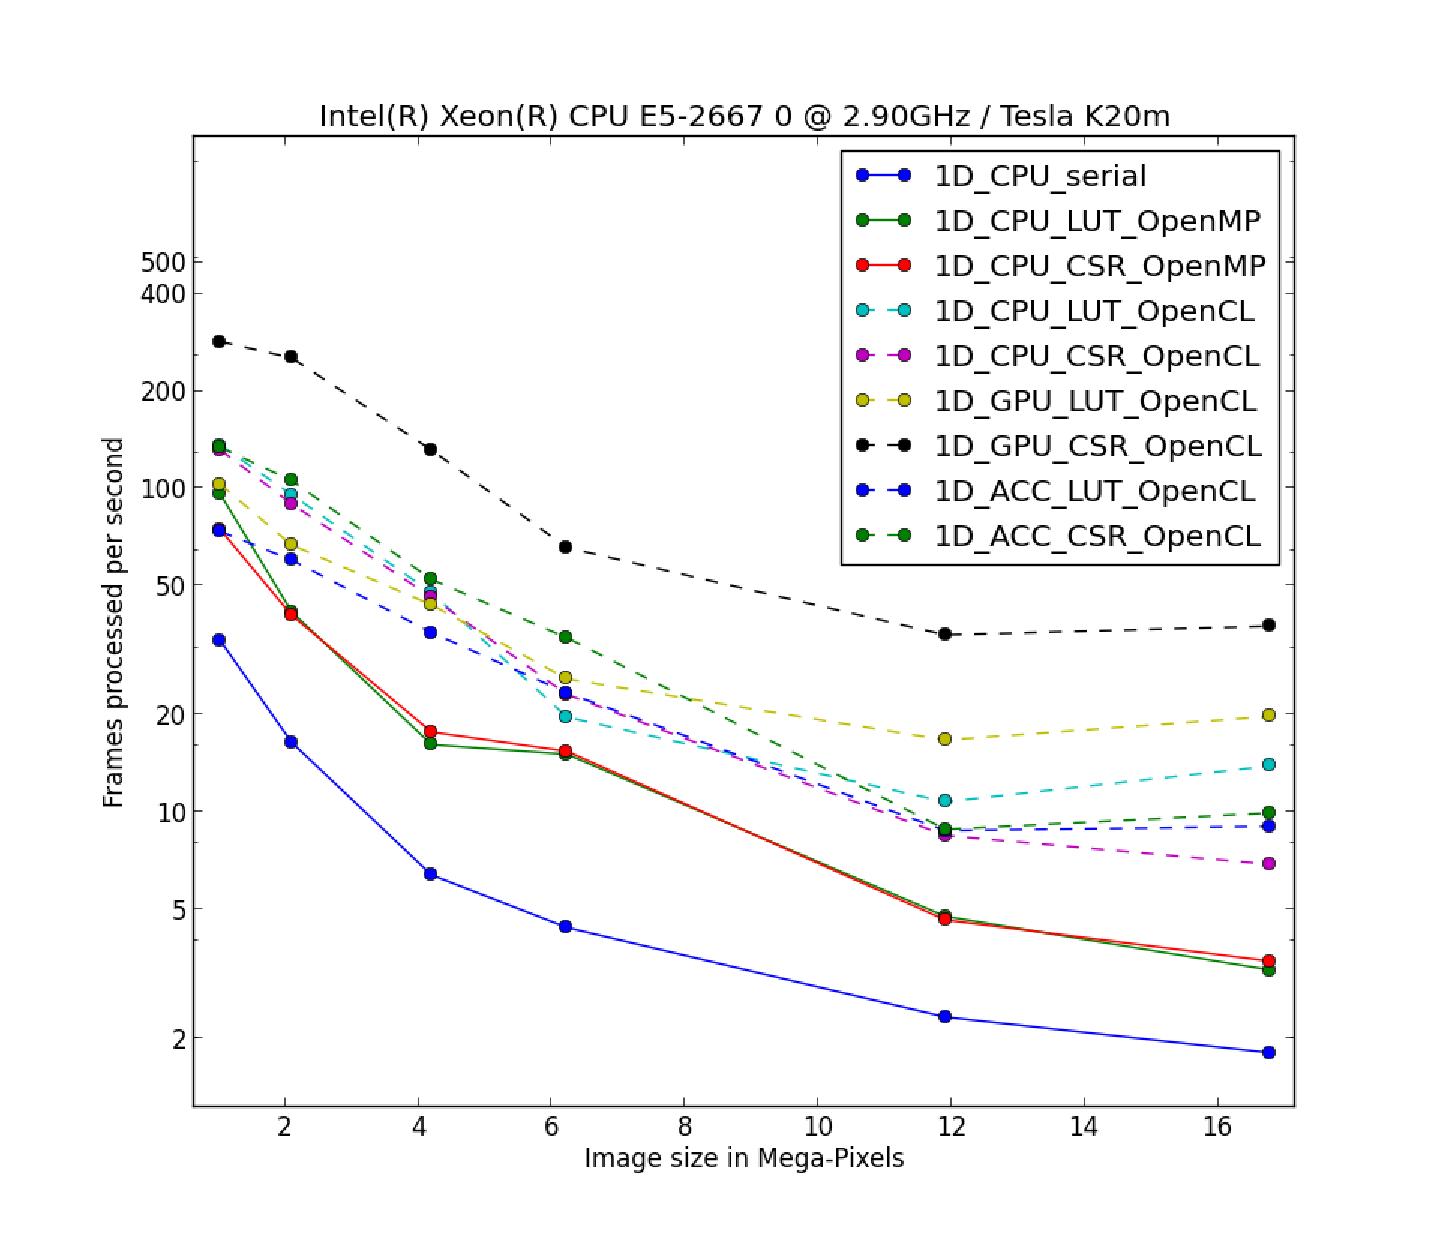
\includegraphics[width=15cm]{benchmark.eps}
\caption{Benchmark of the various algorithm to perform azimuthal integration in
pyFAI}
\end{center}
\end{figure}

In this benchmark, four groups of curves can be extracted.
\begin{itemize}
  \item The lower plain blue curve presenting the serial Cython code using
  histograms (corresponding to the ``splitbbox'' method) which is the slowest
  implementation (even if it is 7x faster than a numpy implementation).
  \item The red and blue plain curves which correspond to the two parallel
  Cython implementation for look-up tables integration.
  \item the group of dashed curves which represent the OpenCL optimized code
  running on the 12 CPU cores, the 60 cores from the accelerator or the GPU (LUT
  implementation).
  \item The upper curve, in dashed black correspond the CSR sparse matrix
  multiplication implemented in OpenCL code and running on the Tesla K20 card
  which is twice faster than any other implementation: a 4096x4096 pixel image
  can be processed in less the 19 milliseconds, which represent 885 Mega-pixels
  per second. This gain in performances is obtained from the collaborative
  partial reduction from all threads within a workgroup.
\end{itemize}


\ack{Acknowledgements}

The authors would like to thank all ESRF beamline teams for supporting the
pyFAI development, especially BM01, ID02, ID11, ID13, ID15, ID23, BM26, ID29, BM29,
ID30. In the instrumentation division (ISDD) we would like to thank Claudio
Ferrero, head of data analysis unit, and Andy G\"otz, head of software group, for
supporting the algorithmic work performed on pyFAI in addition to the features
seen by the user.
V. Armando Solé, the author of PyMca, is also acknowledged for providing us some
important graphical user interface building blocks.

The huge parallelization work on the integration routines and their porting to
manycore devices was mainly done by Dimitris Karkoulis, Zubair Nawaz and Giannis Ashiotis,
thanks the EU-grant LinkSCEEM-2 (RI-261600).

We would like to thank David Flot for the protein
diffraction image with ice-rings (fig. \ref{separate}) and Martha Brennich for
the silver behenate calibration image (fig. \ref{calib}).

\end{document}
